% Options for packages loaded elsewhere
\PassOptionsToPackage{unicode}{hyperref}
\PassOptionsToPackage{hyphens}{url}
%
\documentclass[
  a4paper,
]{article}
\usepackage{amsmath,amssymb}
\usepackage{iftex}
\ifPDFTeX
  \usepackage[T1]{fontenc}
  \usepackage[utf8]{inputenc}
  \usepackage{textcomp} % provide euro and other symbols
\else % if luatex or xetex
  \usepackage{unicode-math} % this also loads fontspec
  \defaultfontfeatures{Scale=MatchLowercase}
  \defaultfontfeatures[\rmfamily]{Ligatures=TeX,Scale=1}
\fi
\usepackage{lmodern}
\ifPDFTeX\else
  % xetex/luatex font selection
    \setmainfont[]{Helvetica}
\fi
% Use upquote if available, for straight quotes in verbatim environments
\IfFileExists{upquote.sty}{\usepackage{upquote}}{}
\IfFileExists{microtype.sty}{% use microtype if available
  \usepackage[]{microtype}
  \UseMicrotypeSet[protrusion]{basicmath} % disable protrusion for tt fonts
}{}
\makeatletter
\@ifundefined{KOMAClassName}{% if non-KOMA class
  \IfFileExists{parskip.sty}{%
    \usepackage{parskip}
  }{% else
    \setlength{\parindent}{0pt}
    \setlength{\parskip}{6pt plus 2pt minus 1pt}}
}{% if KOMA class
  \KOMAoptions{parskip=half}}
\makeatother
\usepackage{xcolor}
\usepackage[margin=0.75in]{geometry}
\usepackage{graphicx}
\makeatletter
\newsavebox\pandoc@box
\newcommand*\pandocbounded[1]{% scales image to fit in text height/width
  \sbox\pandoc@box{#1}%
  \Gscale@div\@tempa{\textheight}{\dimexpr\ht\pandoc@box+\dp\pandoc@box\relax}%
  \Gscale@div\@tempb{\linewidth}{\wd\pandoc@box}%
  \ifdim\@tempb\p@<\@tempa\p@\let\@tempa\@tempb\fi% select the smaller of both
  \ifdim\@tempa\p@<\p@\scalebox{\@tempa}{\usebox\pandoc@box}%
  \else\usebox{\pandoc@box}%
  \fi%
}
% Set default figure placement to htbp
\def\fps@figure{htbp}
\makeatother
\setlength{\emergencystretch}{3em} % prevent overfull lines
\providecommand{\tightlist}{%
  \setlength{\itemsep}{0pt}\setlength{\parskip}{0pt}}
\setcounter{secnumdepth}{-\maxdimen} % remove section numbering
\usepackage{titling}
\pretitle{\begin{flushleft}}
\posttitle{\end{flushleft}}
\usepackage{booktabs}
\usepackage{longtable}
\usepackage{float}
\floatplacement{figure}{H}
\usepackage{colortbl}
\usepackage{pdflscape}
\usepackage{tabu}
\usepackage{makecell}
\usepackage{xcolor}
\usepackage{soul}
\usepackage{caption}
\usepackage[singlelinecheck=false]{caption}
\usepackage[font={small,bf}]{caption}
\usepackage{multirow}
\usepackage{array}
\usepackage{lscape}
\newcommand{\blandscape}{\begin{landscape}}
\newcommand{\elandscape}{\end{landscape}}
\usepackage[dvipsnames]{xcolor}
\renewcommand{\footnotesize}{\tiny}
\usepackage{threeparttable}
\usepackage{booktabs}
\usepackage{longtable}
\usepackage{array}
\usepackage{multirow}
\usepackage{wrapfig}
\usepackage{float}
\usepackage{colortbl}
\usepackage{pdflscape}
\usepackage{tabu}
\usepackage{threeparttable}
\usepackage{threeparttablex}
\usepackage[normalem]{ulem}
\usepackage{makecell}
\usepackage{xcolor}
\usepackage{bookmark}
\IfFileExists{xurl.sty}{\usepackage{xurl}}{} % add URL line breaks if available
\urlstyle{same}
\hypersetup{
  hidelinks,
  pdfcreator={LaTeX via pandoc}}

\title{\vspace{-1.5cm} \begin{LARGE} WGS Quality Control Report \end{LARGE}}
\author{}
\date{\vspace{-2.5em}}

\begin{document}
\maketitle

\normalsize Batch Name: 2025-06-20\_P

\normalsize Experiment Name: 25ARS\_KPNGHRU\_LYCVL

\fontsize{7}{8}
\selectfont
\captionsetup[table]{labelformat=empty}
\renewcommand{\arraystretch}{1.2}

\begin{longtable}[t]{>{\centering\arraybackslash}p{1cm}>{\centering\arraybackslash}p{2.8cm}>{\centering\arraybackslash}p{1.5cm}>{\centering\arraybackslash}p{5cm}>{\centering\arraybackslash}p{5cm}}
\toprule
\multicolumn{1}{>{\centering\arraybackslash}p{1cm}}{\cellcolor[HTML]{D4D4D4}{\textbf{Isolate No.}}} & \multicolumn{1}{>{\centering\arraybackslash}p{2.8cm}}{\cellcolor[HTML]{D4D4D4}{\textbf{Sample ID}}} & \multicolumn{1}{>{\centering\arraybackslash}p{1.5cm}}{\cellcolor[HTML]{D4D4D4}{\textbf{Description}}} & \multicolumn{1}{>{\centering\arraybackslash}p{5cm}}{\cellcolor[HTML]{D4D4D4}{\textbf{ARSRL}}} & \multicolumn{1}{>{\centering\arraybackslash}p{5cm}}{\cellcolor[HTML]{D4D4D4}{\textbf{WGS}}}\\
\midrule
1 & 24ARS\_BRH0194 & UDI129 & \em{Klebsiella pneumoniae} & \em{Klebsiella pneumoniae}\\
2 & 24ARS\_DMC0493 & UDI149 & \em{Klebsiella pneumoniae} & \em{Klebsiella pneumoniae}\\
3 & 24ARS\_JLM0260 & UDI133 & \em{Klebsiella pneumoniae} & \em{Klebsiella pneumoniae}\\
4 & 24ARS\_JLM0261 & UDI134 & \em{Klebsiella pneumoniae} & \em{Klebsiella pneumoniae}\\
5 & 24ARS\_NKI0073 & UDI154 & \em{Klebsiella pneumoniae} & \em{Klebsiella pneumoniae}\\
\addlinespace
6 & 24ARS\_SLH0180 & UDI158 & \em{Klebsiella pneumoniae} & \em{Klebsiella pneumoniae}\\
7 & 24ARS\_SLH0226 & UDI131 & \em{Klebsiella pneumoniae} & \em{Klebsiella pneumoniae}\\
\cellcolor[HTML]{FD7979}{8} & \cellcolor[HTML]{FD7979}{24ARS\_STU0113} & \cellcolor[HTML]{FD7979}{UDI159} & \cellcolor[HTML]{FD7979}{\em{Klebsiella pneumoniae}} & \cellcolor[HTML]{FD7979}{\em{Klebsiella pneumoniae}}\\
9 & 24ARS\_JLM0232 & UDI121 & \em{Klebsiella pneumoniae} & \em{Klebsiella pneumoniae}\\
\cellcolor[HTML]{FD7979}{10} & \cellcolor[HTML]{FD7979}{24ARS\_VSM0585} & \cellcolor[HTML]{FD7979}{UDI122} & \cellcolor[HTML]{FD7979}{\em{Klebsiella pneumoniae}} & \cellcolor[HTML]{FD7979}{\em{Klebsiella pneumoniae}}\\
\addlinespace
\cellcolor[HTML]{FD7979}{11} & \cellcolor[HTML]{FD7979}{24ARS\_VSM0587} & \cellcolor[HTML]{FD7979}{UDI124} & \cellcolor[HTML]{FD7979}{\em{Klebsiella pneumoniae}} & \cellcolor[HTML]{FD7979}{\em{Klebsiella pneumoniae}}\\
12 & 24ARS\_VSM0589 & UDI126 & \em{Klebsiella pneumoniae} & \em{Klebsiella pneumoniae}\\
13 & 24ARS\_STU0114 & UDI160 & \em{Klebsiella pneumoniae} & \em{Klebsiella pneumoniae}\\
\cellcolor[HTML]{FD7979}{14} & \cellcolor[HTML]{FD7979}{24ARS\_VSM0661} & \cellcolor[HTML]{FD7979}{UDI138} & \cellcolor[HTML]{FD7979}{\em{Klebsiella pneumoniae}} & \cellcolor[HTML]{FD7979}{\em{Klebsiella pneumoniae}}\\
15 & 24ARS\_VSM0663 & UDI140 & \em{Klebsiella pneumoniae} & \em{Klebsiella pneumoniae}\\
\addlinespace
16 & 25ARS\_BGH0042 & UDI141 & \em{Klebsiella pneumoniae} & \em{Klebsiella pneumoniae}\\
17 & 25ARS\_MAR0002 & UDI143 & \em{Klebsiella pneumoniae} & \em{Klebsiella pneumoniae}\\
18 & 24ARS\_NKI0076 & UDI156 & \em{Klebsiella pneumoniae} & \em{Klebsiella quasipneumoniae}\\
19 & 24ARS\_VSM0659 & UDI136 & \em{Klebsiella pneumoniae} & \em{Klebsiella quasipneumoniae}\\
20 & 24ARS\_VSM0588 & UDI125 & \em{Klebsiella pneumoniae (x)} & \em{NA}\\
\bottomrule
\multicolumn{5}{l}{\rule{0pt}{1em}\textit{Legend:} PASS   |   \colorbox{Salmon}{FAILURE}   |   \textcolor{Blue}{EXCEEDS THRESHOLD METRIC/S}   |   (x) - NON-CONCORDANT   |}\\
\end{longtable}

\fontsize{7}{8}
\selectfont
\captionsetup[table]{labelformat=empty}
\renewcommand{\arraystretch}{1.2}

\begin{tabular}{>{\centering\arraybackslash}p{3cm}>{\centering\arraybackslash}p{3cm}>{\centering\arraybackslash}p{7cm}}
\toprule
\multicolumn{3}{l}{\textbf{Sample excluded in the analysis}} \\
\cmidrule(l{3pt}r{3pt}){1-3}
\multicolumn{1}{>{\centering\arraybackslash}p{3cm}}{\cellcolor[HTML]{D4D4D4}{\textbf{Sample ID}}} & \multicolumn{1}{>{\centering\arraybackslash}p{3cm}}{\cellcolor[HTML]{D4D4D4}{\textbf{Description}}} & \multicolumn{1}{>{\centering\arraybackslash}p{7cm}}{\cellcolor[HTML]{D4D4D4}{\textbf{Remarks}}}\\
\midrule
25ARS\_VC00292\_20250620P & UDI164 & low read count\\
\bottomrule
\end{tabular}

\(\\\) \newpage

\begin{landscape}
\fontsize{7}{8}
\selectfont
\captionsetup[table]{labelformat=empty}
\renewcommand{\arraystretch}{1.2}

\begin{table}[!h]
\centering
\resizebox{\ifdim\width>\linewidth\linewidth\else\width\fi}{!}{
\begin{tabular}{cc>{}ccccccccc}
\toprule
\cellcolor[HTML]{D4D4D4}{\textbf{Isolate No.}} & \cellcolor[HTML]{D4D4D4}{\textbf{Sample ID}} & \cellcolor[HTML]{D4D4D4}{\textbf{WGS ID}} & \cellcolor[HTML]{D4D4D4}{\textbf{completeness}} & \cellcolor[HTML]{D4D4D4}{\textbf{contamination}} & \cellcolor[HTML]{D4D4D4}{\textbf{Depth of coverage}} & \cellcolor[HTML]{D4D4D4}{\textbf{Genome size}} & \cellcolor[HTML]{D4D4D4}{\textbf{GC content}} & \cellcolor[HTML]{D4D4D4}{\textbf{Contig count}} & \cellcolor[HTML]{D4D4D4}{\textbf{N50}} & \cellcolor[HTML]{D4D4D4}{\textbf{Mean read Q-score}}\\
\midrule
1 & 24ARS\_BRH0194 & \em{Klebsiella pneumoniae} & 100 & 0.24 & 41.3 & 5.60 Mb & 57 & 55 & 307369 & 36.4\\
2 & 24ARS\_DMC0493 & \em{Klebsiella pneumoniae} & 100 & 0.14 & 62.0 & 5.53 Mb & 57 & 70 & 228881 & 36.5\\
3 & 24ARS\_JLM0260 & \em{Klebsiella pneumoniae} & 100 & 0.21 & 77.3 & 5.57 Mb & 57 & 71 & 288047 & 36.5\\
4 & 24ARS\_JLM0261 & \em{Klebsiella pneumoniae} & 100 & 0.07 & 22.2 & 5.63 Mb & 57 & 144 & 161871 & 36.3\\
5 & 24ARS\_NKI0073 & \em{Klebsiella pneumoniae} & 100 & 0.32 & 26.0 & 5.44 Mb & 57 & 86 & 266544 & 36.5\\
\addlinespace
6 & 24ARS\_SLH0180 & \em{Klebsiella pneumoniae} & 100 & 1.15 & 41.7 & 5.61 Mb & 57 & 63 & 289355 & 36.3\\
7 & 24ARS\_SLH0226 & \em{Klebsiella pneumoniae} & 100 & 2.46 & 58.0 & 5.72 Mb & 57 & 75 & 288283 & 36.4\\
\cellcolor[HTML]{FD7979}{8} & \cellcolor[HTML]{FD7979}{24ARS\_STU0113} & \em{\cellcolor[HTML]{FD7979}{Klebsiella pneumoniae}} & \cellcolor[HTML]{FD7979}{100} & \cellcolor[HTML]{FD7979}{0.22} & \cellcolor[HTML]{FD7979}{\textcolor{blue}{\textbf{15.7}}} & \cellcolor[HTML]{FD7979}{5.16 Mb} & \cellcolor[HTML]{FD7979}{58} & \cellcolor[HTML]{FD7979}{133} & \cellcolor[HTML]{FD7979}{99483} & \cellcolor[HTML]{FD7979}{36.6}\\
9 & 24ARS\_JLM0232 & \em{Klebsiella pneumoniae} & 100 & 0.13 & 70.1 & 5.15 Mb & 58 & 42 & 241253 & 36.5\\
\cellcolor[HTML]{FD7979}{10} & \cellcolor[HTML]{FD7979}{24ARS\_VSM0585} & \em{\cellcolor[HTML]{FD7979}{Klebsiella pneumoniae}} & \cellcolor[HTML]{FD7979}{100} & \cellcolor[HTML]{FD7979}{1.83} & \cellcolor[HTML]{FD7979}{\textcolor{blue}{\textbf{13.5}}} & \cellcolor[HTML]{FD7979}{5.73 Mb} & \cellcolor[HTML]{FD7979}{57} & \cellcolor[HTML]{FD7979}{304} & \cellcolor[HTML]{FD7979}{41150} & \cellcolor[HTML]{FD7979}{36.4}\\
\addlinespace
\cellcolor[HTML]{FD7979}{11} & \cellcolor[HTML]{FD7979}{24ARS\_VSM0587} & \em{\cellcolor[HTML]{FD7979}{Klebsiella pneumoniae}} & \cellcolor[HTML]{FD7979}{100} & \cellcolor[HTML]{FD7979}{0.18} & \cellcolor[HTML]{FD7979}{\textcolor{blue}{\textbf{15.4}}} & \cellcolor[HTML]{FD7979}{5.57 Mb} & \cellcolor[HTML]{FD7979}{57} & \cellcolor[HTML]{FD7979}{159} & \cellcolor[HTML]{FD7979}{69362} & \cellcolor[HTML]{FD7979}{36.5}\\
12 & 24ARS\_VSM0589 & \em{Klebsiella pneumoniae} & 100 & 0.18 & 59.6 & 5.18 Mb & 58 & 36 & 367180 & 36.5\\
13 & 24ARS\_STU0114 & \em{Klebsiella pneumoniae} & 100 & 0.2 & 31.2 & 5.50 Mb & 57 & 67 & 324617 & 36.5\\
\cellcolor[HTML]{FD7979}{14} & \cellcolor[HTML]{FD7979}{24ARS\_VSM0661} & \em{\cellcolor[HTML]{FD7979}{Klebsiella pneumoniae}} & \cellcolor[HTML]{FD7979}{100} & \cellcolor[HTML]{FD7979}{0.2} & \cellcolor[HTML]{FD7979}{\textcolor{blue}{\textbf{18.6}}} & \cellcolor[HTML]{FD7979}{5.58 Mb} & \cellcolor[HTML]{FD7979}{57} & \cellcolor[HTML]{FD7979}{159} & \cellcolor[HTML]{FD7979}{93286} & \cellcolor[HTML]{FD7979}{36.5}\\
15 & 24ARS\_VSM0663 & \em{Klebsiella pneumoniae} & 100 & 1.96 & 22.7 & 5.62 Mb & 57 & 221 & 55603 & 36.5\\
\addlinespace
16 & 25ARS\_BGH0042 & \em{Klebsiella pneumoniae} & 100 & 0.65 & 36.1 & 5.66 Mb & 57 & 83 & 304522 & 36.4\\
17 & 25ARS\_MAR0002 & \em{Klebsiella pneumoniae} & 100 & 0.17 & 65.5 & 5.42 Mb & 57 & 86 & 312797 & 36.4\\
18 & 24ARS\_NKI0076 & \em{Klebsiella quasipneumoniae} & 100 & 0.12 & 70.1 & 5.38 Mb & 58 & 60 & 280597 & 36.5\\
19 & 24ARS\_VSM0659 & \em{Klebsiella quasipneumoniae} & 100 & 0.07 & 32.8 & 5.36 Mb & 58 & 42 & 339417 & 36.4\\
\bottomrule
\multicolumn{11}{l}{\rule{0pt}{1em}\textit{Legend:} PASS   |   \colorbox{Salmon}{FAILURE}   |   \textcolor{Blue}{EXCEEDS THRESHOLD METRIC/S}   |   (x) - NON-CONCORDANT   |}\\
\end{tabular}}
\end{table}









$\\$ $\\$ $\\$ $\color{red}{\normalsize\textbf{RECOMMENDATION:}}$



\begin{tabular}{>{\raggedright\arraybackslash}p{6cm}>{\centering\arraybackslash}p{6cm}>{\centering\arraybackslash}p{4cm}}
\toprule
\cellcolor[HTML]{D4D4D4}{\textbf{Sample ID}} & \cellcolor[HTML]{D4D4D4}{\textbf{Reason - Failed Metrics}} & \cellcolor[HTML]{D4D4D4}{\textbf{Remarks}}\\
\midrule
\cellcolor{gray!10}{24ARS\_STU0113, 24ARS\_VSM0585, 24ARS\_VSM0587, 24ARS\_VSM0661} & \cellcolor{gray!10}{Depth of coverage} & \cellcolor{gray!10}{For repeat testing}\\
\bottomrule
\end{tabular}



\end{landscape}

\fontsize{7}{8}
\selectfont
\captionsetup[table]{labelformat=empty}
\renewcommand{\arraystretch}{1.2}

\begin{longtable}[l]{>{\raggedright\arraybackslash}p{8cm}c}
\toprule
\cellcolor[HTML]{D4D4D4}{\textbf{WGS\_ID}} & \cellcolor[HTML]{D4D4D4}{\textbf{Number}}\\
\midrule
\em{Klebsiella pneumoniae} & 17\\
\em{Klebsiella quasipneumoniae} & 2\\
\bottomrule
\end{longtable}

\begin{itemize}
\item
  \(\color{red}2\) distinct species were identified among
  \(\color{red}20\) isolates.
\item
  \(\color{red}75.00\) \% (n=15) of the isolates passed the QC, while
  \(\color{red}20.00\) \% (n=4) were tagged with failure.
\item
  Concordance between ARSRL and WGS species report was
  \(\color{red}95.00\) \%. \(\\\)
\end{itemize}

\subsubsection{GRAPHS}\label{graphs}

\fontsize{7}{8}
\selectfont
\captionsetup[table]{labelformat=empty}
\renewcommand{\arraystretch}{1.2}

\pandocbounded{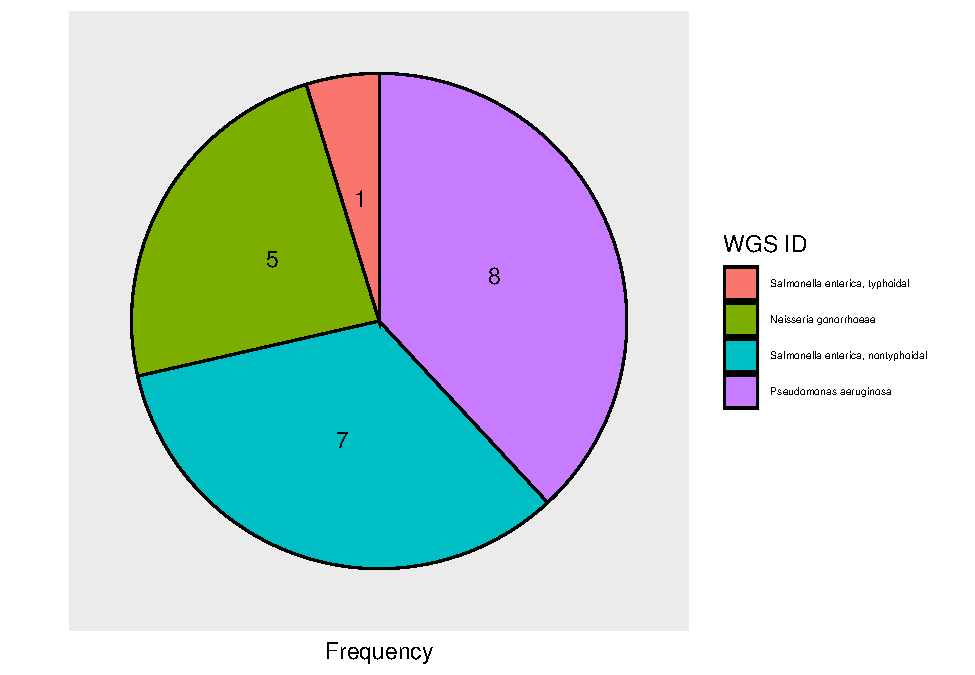
\includegraphics[keepaspectratio]{qualifyr_report_2025-06-20_P_files/figure-latex/pie_chart-1.pdf}}

\subsubsection{Result Classification}\label{result-classification}

\pandocbounded{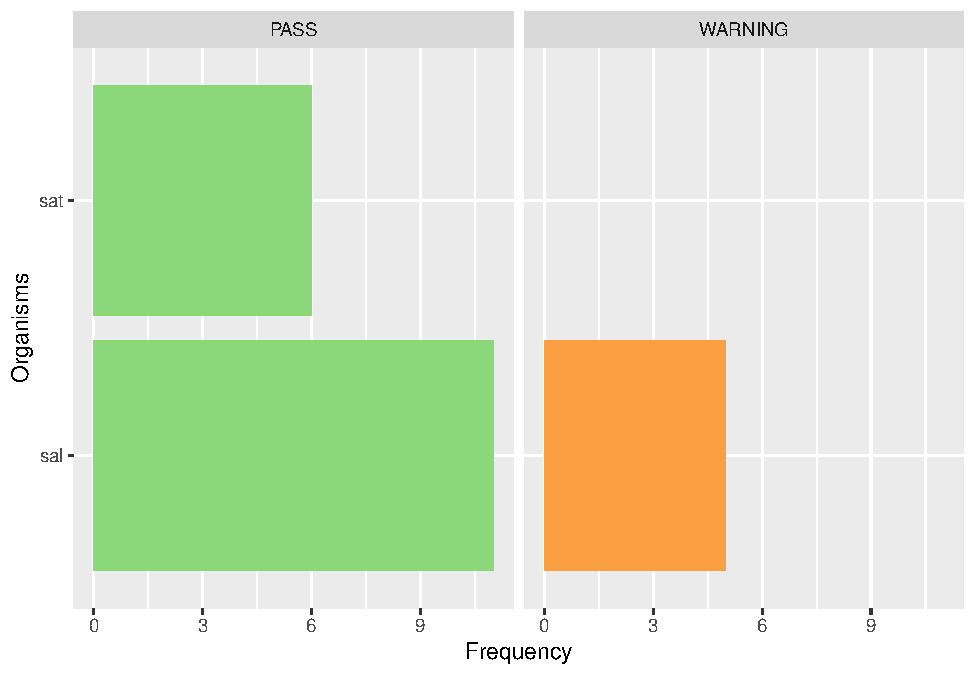
\includegraphics[keepaspectratio]{qualifyr_report_2025-06-20_P_files/figure-latex/organism results-1.pdf}}

\subsubsection{Number of contigs}\label{number-of-contigs}

\pandocbounded{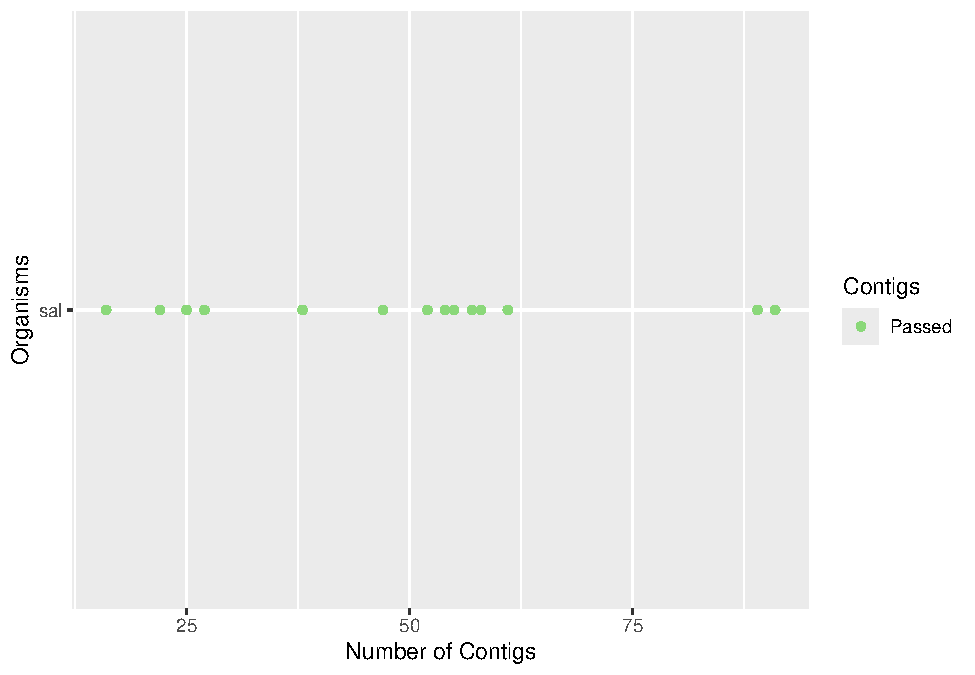
\includegraphics[keepaspectratio]{qualifyr_report_2025-06-20_P_files/figure-latex/unnamed-chunk-1-1.pdf}}

\subsubsection{N50 Value}\label{n50-value}

\pandocbounded{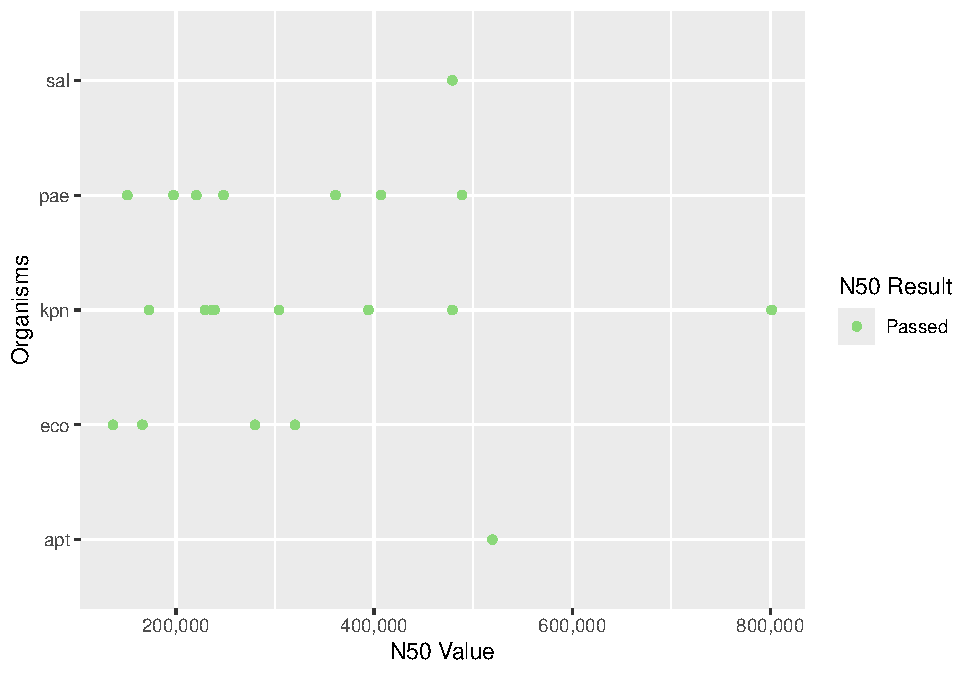
\includegraphics[keepaspectratio]{qualifyr_report_2025-06-20_P_files/figure-latex/n50_result -1.pdf}}

\subsubsection{Total Length}\label{total-length}

\pandocbounded{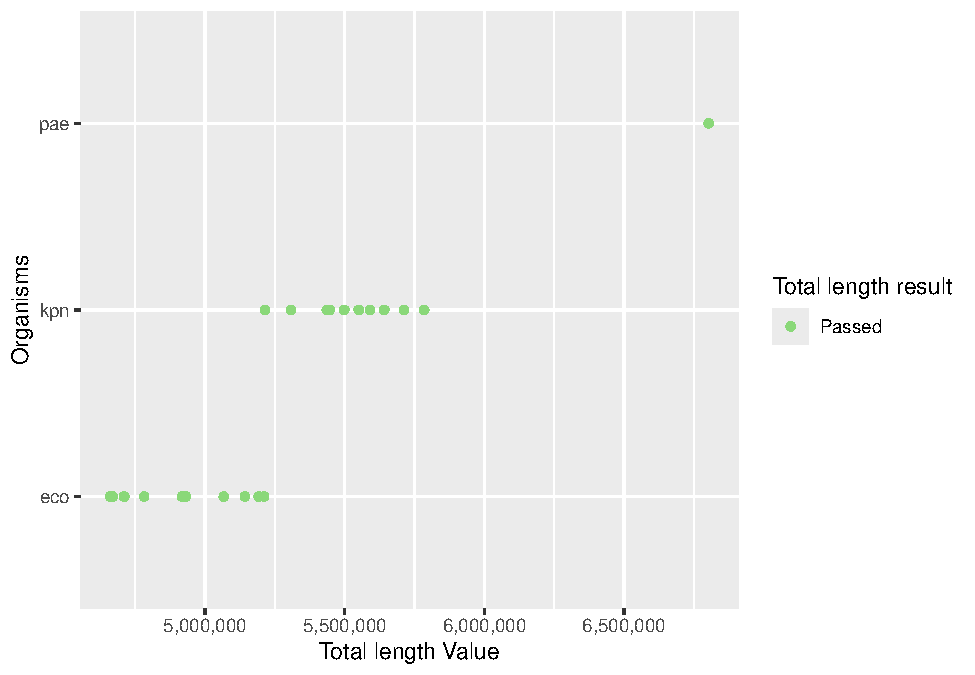
\includegraphics[keepaspectratio]{qualifyr_report_2025-06-20_P_files/figure-latex/length_result -1.pdf}}

\fontsize{7}{8}
\selectfont
\captionsetup[table]{labelformat=empty}
\renewcommand{\arraystretch}{1}

\subsubsection{MLST RESULTS}\label{mlst-results}

\begin{longtable}[l]{>{\centering\arraybackslash}p{3cm}>{\centering\arraybackslash}p{3cm}>{\centering\arraybackslash}p{1cm}>{\centering\arraybackslash}p{1cm}>{\centering\arraybackslash}p{1cm}>{\centering\arraybackslash}p{1cm}>{\centering\arraybackslash}p{1cm}>{\centering\arraybackslash}p{1cm}>{\centering\arraybackslash}p{1cm}>{\centering\arraybackslash}p{1cm}}
\toprule
\cellcolor[HTML]{D4D4D4}{\textbf{sample\_id}} & \cellcolor[HTML]{D4D4D4}{\textbf{species}} & \cellcolor[HTML]{D4D4D4}{\textbf{MLST}} & \cellcolor[HTML]{D4D4D4}{\textbf{gapA}} & \cellcolor[HTML]{D4D4D4}{\textbf{infB}} & \cellcolor[HTML]{D4D4D4}{\textbf{mdh}} & \cellcolor[HTML]{D4D4D4}{\textbf{pgi}} & \cellcolor[HTML]{D4D4D4}{\textbf{phoE}} & \cellcolor[HTML]{D4D4D4}{\textbf{rpoB}} & \cellcolor[HTML]{D4D4D4}{\textbf{tonB}}\\
\midrule
24ARS\_BRH0194 & \em{Klebsiella pneumoniae} & 23 & 2 & 1 & 1 & 1 & 9 & 4 & 12\\
24ARS\_DMC0493 & \em{Klebsiella pneumoniae} & 4813 & 4 & 1 & 1 & 1 & 1 & 272 & 35\\
24ARS\_JLM0232 & \em{Klebsiella pneumoniae} & 1408 & 2 & 9 & 1 & 1 & 4 & 4 & 129\\
24ARS\_JLM0260 & \em{Klebsiella pneumoniae} & 147 & 3 & 4 & 6 & 1 & 7 & 4 & 38\\
24ARS\_JLM0261 & \em{Klebsiella pneumoniae} & 15 & 1 & 1 & 1 & 1 & 1 & 1 & 1\\
\addlinespace
24ARS\_NKI0073 & \em{Klebsiella pneumoniae} & 86 & 9 & 4 & 2 & 1 & 1 & 1 & 27\\
24ARS\_NKI0076 & \em{Klebsiella quasipneumoniae} & 2660 & 17 & 19 & 39 & 20 & 156 & 21 & 52\\
24ARS\_SLH0180 & \em{Klebsiella pneumoniae} & 23 & 2 & 1 & 1 & 1 & 9 & 4 & 12\\
24ARS\_SLH0226 & \em{Klebsiella pneumoniae} & 147 & 3 & 4 & 6 & 1 & 7 & 4 & 38\\
24ARS\_STU0113 & \em{Klebsiella pneumoniae} & 281 & 7 & 1 & 5 & 46 & 1 & 1 & 84\\
\addlinespace
24ARS\_STU0114 & \em{Klebsiella pneumoniae} & 86 & 9 & 4 & 2 & 1 & 1 & 1 & 27\\
24ARS\_VSM0585 & \em{Klebsiella pneumoniae} & 893 & 25 & 1 & 101 & 1 & 10 & 1 & 100\\
24ARS\_VSM0587 & \em{Klebsiella pneumoniae} & 147 & 3 & 4 & 6 & 1 & 7 & 4 & 38\\
24ARS\_VSM0589 & \em{Klebsiella pneumoniae} & 753 & 14 & 1 & 2 & 1 & 135 & 4 & 12\\
24ARS\_VSM0659 & \em{Klebsiella quasipneumoniae} & 3864 & 18 & 71 & 281 & 59 & 31 & 92 & 50\\
\addlinespace
24ARS\_VSM0661 & \em{Klebsiella pneumoniae} & 1 & 4 & 4 & 1 & 1 & 7 & 4 & 10\\
24ARS\_VSM0663 & \em{Klebsiella pneumoniae} & 147 & 3 & 4 & 6 & 1 & 7 & 4 & 38\\
25ARS\_BGH0042 & \em{Klebsiella pneumoniae} & 147 & 3 & 4 & 6 & 1 & 7 & 4 & 38\\
25ARS\_MAR0002 & \em{Klebsiella pneumoniae} & 656 & 4 & 4 & 1 & 1 & 7 & 4 & 4\\
\bottomrule
\multicolumn{10}{l}{\rule{0pt}{1em}\textit{Legend: } (-) Not identified}\\
\end{longtable}

\subsubsection{MLST RESULTS SUMMARY:}\label{mlst-results-summary}

\begin{longtable}[l]{>{\raggedright\arraybackslash}p{6cm}>{\raggedright\arraybackslash}p{10cm}}
\toprule
\cellcolor[HTML]{D4D4D4}{\textbf{wgs\_id}} & \cellcolor[HTML]{D4D4D4}{\textbf{mlst\_count}}\\
\midrule
\em{Klebsiella pneumoniae} & 23 (n= 2 ), 4813 (n= 1 ), 1408 (n= 1 ), 147 (n= 5 ), 15 (n= 1 ), 86 (n= 2 ), 281 (n= 1 ), 893 (n= 1 ), 753 (n= 1 ), 1 (n= 1 ), 656 (n= 1 )\\
\em{Klebsiella quasipneumoniae} & 2660 (n= 1 ), 3864 (n= 1 )\\
\bottomrule
\multicolumn{2}{l}{\rule{0pt}{1em}\textit{Legend: } (-) Not identified}\\
\end{longtable}

\newpage
\begin{landscape}
\fontsize{7}{8}
\selectfont
\captionsetup[table]{labelformat=empty}
\renewcommand{\arraystretch}{1.2}


\normalsize\textbf{AMR PREDICTION RESULTS}\textbf\normalsize




\fontsize{7}{8}
\selectfont
\captionsetup[table]{labelformat=empty}
\renewcommand{\arraystretch}{1.2}

\begingroup\fontsize{7}{9}\selectfont

\resizebox{\ifdim\width>\linewidth\linewidth\else\width\fi}{!}{
\begin{tabular}{c>{\centering\arraybackslash}p{3cm}>{\centering\arraybackslash}p{3cm}>{\centering\arraybackslash}p{3cm}>{\centering\arraybackslash}p{3cm}>{\centering\arraybackslash}p{3cm}>{\centering\arraybackslash}p{3cm}}
\toprule
\multicolumn{7}{l}{\textbf{\textit{Klebsiella pneumoniae} (Part 1.1)}} \\
\cmidrule(l{3pt}r{3pt}){1-7}
\cellcolor[HTML]{D4D4D4}{\textbf{sample\_id}} & \cellcolor[HTML]{D4D4D4}{\textbf{AMR AMIKACIN/ KAMYCIN}} & \cellcolor[HTML]{D4D4D4}{\textbf{AMR AMIKACIN/ KAMYCIN/ QUINOLONE/ TOBRAMYCIN}} & \cellcolor[HTML]{D4D4D4}{\textbf{AMR AMINOGLYCOSIDE}} & \cellcolor[HTML]{D4D4D4}{\textbf{AMR AZITHROMYCIN/ ERYTHROMYCIN/ SPIRAMYCIN/ TELITHROMYCIN}} & \cellcolor[HTML]{D4D4D4}{\textbf{AMR BETA-LACTAM}} & \cellcolor[HTML]{D4D4D4}{\textbf{AMR BLEOMYCIN}}\\
\midrule
24ARS\_BRH0194 & NA & NA & NA & NA & blaSHV-11 & NA\\
24ARS\_DMC0493 & NA & aac(6')-Ib-cr5 & NA & mph(A) & blaTEM-1, blaSHV-1 & NA\\
24ARS\_JLM0232 & NA & NA & NA & NA & blaSHV-11 & NA\\
24ARS\_JLM0260 & NA & aac(6')-Ib-cr5 & NA & NA & blaSHV-11, blaTEM-1 & ble\\
24ARS\_JLM0261 & NA & aac(6')-Ib-cr5 & NA & mph(A) & blaTEM, blaSHV-28 & ble\\
\addlinespace
24ARS\_NKI0073 & NA & NA & NA & NA & blaSHV-1 & NA\\
\bottomrule
\end{tabular}}
\endgroup{}


\vspace{5mm}

\begingroup\fontsize{7}{9}\selectfont

\resizebox{\ifdim\width>\linewidth\linewidth\else\width\fi}{!}{
\begin{tabular}{c>{\centering\arraybackslash}p{3cm}>{\centering\arraybackslash}p{3cm}>{\centering\arraybackslash}p{3cm}>{\centering\arraybackslash}p{3cm}>{\centering\arraybackslash}p{3cm}>{\centering\arraybackslash}p{3cm}}
\toprule
\multicolumn{7}{l}{\textbf{\textit{Klebsiella pneumoniae} (Part 1.2)}} \\
\cmidrule(l{3pt}r{3pt}){1-7}
\cellcolor[HTML]{D4D4D4}{\textbf{sample\_id}} & \cellcolor[HTML]{D4D4D4}{\textbf{AMR CARBAPENEM}} & \cellcolor[HTML]{D4D4D4}{\textbf{AMR CEPHALOSPORIN}} & \cellcolor[HTML]{D4D4D4}{\textbf{AMR CHLORAMPHENICOL}} & \cellcolor[HTML]{D4D4D4}{\textbf{AMR CHLORAMPHENICOL/ FLORFENICOL}} & \cellcolor[HTML]{D4D4D4}{\textbf{AMR CLINDAMYCIN/ ERYTHROMYCIN}} & \cellcolor[HTML]{D4D4D4}{\textbf{AMR CLINDAMYCIN/ ERYTHROMYCIN/ STREPTOGRAMIN B}}\\
\midrule
24ARS\_BRH0194 & NA & NA & NA & NA & NA & NA\\
24ARS\_DMC0493 & NA & blaCTX-M-15 & NA & NA & NA & NA\\
24ARS\_JLM0232 & NA & NA & NA & NA & NA & NA\\
24ARS\_JLM0260 & blaNDM-7 & blaCTX-M-15, blaOXA-1 & catB3 & NA & NA & erm(B)\\
24ARS\_JLM0261 & blaNDM-7 & blaOXA-1, blaCTX-M-15 & catB3 & NA & NA & NA\\
\addlinespace
24ARS\_NKI0073 & NA & NA & NA & NA & NA & NA\\
\bottomrule
\end{tabular}}
\endgroup{}


\vspace{5mm}

\begingroup\fontsize{7}{9}\selectfont

\resizebox{\ifdim\width>\linewidth\linewidth\else\width\fi}{!}{
\begin{tabular}{c>{\centering\arraybackslash}p{3cm}>{\centering\arraybackslash}p{3cm}>{\centering\arraybackslash}p{3cm}>{\centering\arraybackslash}p{3cm}>{\centering\arraybackslash}p{3cm}>{\centering\arraybackslash}p{3cm}}
\toprule
\multicolumn{7}{l}{\textbf{\textit{Klebsiella pneumoniae} (Part 1.3)}} \\
\cmidrule(l{3pt}r{3pt}){1-7}
\cellcolor[HTML]{D4D4D4}{\textbf{sample\_id}} & \cellcolor[HTML]{D4D4D4}{\textbf{AMR EFFLUX}} & \cellcolor[HTML]{D4D4D4}{\textbf{AMR FOSFOMYCIN}} & \cellcolor[HTML]{D4D4D4}{\textbf{AMR GENTAMICIN}} & \cellcolor[HTML]{D4D4D4}{\textbf{AMR KAMYCIN}} & \cellcolor[HTML]{D4D4D4}{\textbf{AMR PHENICOL/ QUINOLONE}} & \cellcolor[HTML]{D4D4D4}{\textbf{AMR QUINOLONE}}\\
\midrule
24ARS\_BRH0194 & kdeA, emrD & fosA & NA & NA & oqxA, oqxB19 & NA\\
24ARS\_DMC0493 & emrD, kdeA & NA & NA & NA & oqxB, oqxA & NA\\
24ARS\_JLM0232 & kdeA, emrD & fosA10 & NA & NA & oqxA, oqxB & NA\\
24ARS\_JLM0260 & kdeA, emrD & fosA & aac(3)-IIe & NA & oqxA, oqxB & qnrS1, qnrB1\\
24ARS\_JLM0261 & emrD, kdeA & fosA & aac(3)-IId & aph(3')-Ia & oqxA, oqxB & qnrB6, qnrS1\\
\addlinespace
24ARS\_NKI0073 & kdeA, emrD & fosA10 & NA & NA & oqxA11, oqxB19 & NA\\
\bottomrule
\end{tabular}}
\endgroup{}


\vspace{5mm}

\begingroup\fontsize{7}{9}\selectfont

\resizebox{\ifdim\width>\linewidth\linewidth\else\width\fi}{!}{
\begin{tabular}{c>{\centering\arraybackslash}p{3cm}>{\centering\arraybackslash}p{3cm}>{\centering\arraybackslash}p{3cm}>{\centering\arraybackslash}p{3cm}>{\centering\arraybackslash}p{3cm}>{\centering\arraybackslash}p{3cm}}
\toprule
\multicolumn{7}{l}{\textbf{\textit{Klebsiella pneumoniae} (Part 1.4)}} \\
\cmidrule(l{3pt}r{3pt}){1-7}
\cellcolor[HTML]{D4D4D4}{\textbf{sample\_id}} & \cellcolor[HTML]{D4D4D4}{\textbf{AMR RIFAMYCIN}} & \cellcolor[HTML]{D4D4D4}{\textbf{AMR STREPTOMYCIN}} & \cellcolor[HTML]{D4D4D4}{\textbf{AMR SULFOMIDE}} & \cellcolor[HTML]{D4D4D4}{\textbf{AMR TETRACYCLINE}} & \cellcolor[HTML]{D4D4D4}{\textbf{AMR TRIMETHOPRIM}} & \cellcolor[HTML]{D4D4D4}{\textbf{STRESS }}\\
\midrule
24ARS\_BRH0194 & NA & NA & NA & NA & NA & asr, fieF\\
24ARS\_DMC0493 & arr-3 & aadA16 & sul1 & tet(A) & dfrA27 & fieF, hsp20, clpK\\
24ARS\_JLM0232 & NA & NA & NA & NA & NA & fieF\\
24ARS\_JLM0260 & NA & aph(3'')-Ib, aph(6)-Id & sul2 & tet(A) & dfrA14 & fieF, clpK, hsp20\\
24ARS\_JLM0261 & arr-3 & aadA16, aadA2 & sul1, sul1 & tet(A) & dfrA27, dfrA12 & clpK, hsp20, fieF, asr\\
\addlinespace
24ARS\_NKI0073 & NA & NA & NA & NA & NA & asr, fieF\\
\bottomrule
\end{tabular}}
\endgroup{}


\vspace{5mm}

\begingroup\fontsize{7}{9}\selectfont

\resizebox{\ifdim\width>\linewidth\linewidth\else\width\fi}{!}{
\begin{tabular}{c>{\centering\arraybackslash}p{3cm}>{\centering\arraybackslash}p{3cm}>{\centering\arraybackslash}p{3cm}>{\centering\arraybackslash}p{3cm}>{\centering\arraybackslash}p{3cm}>{\centering\arraybackslash}p{3cm}}
\toprule
\multicolumn{7}{l}{\textbf{\textit{Klebsiella pneumoniae} (Part 1.5)}} \\
\cmidrule(l{3pt}r{3pt}){1-7}
\cellcolor[HTML]{D4D4D4}{\textbf{sample\_id}} & \cellcolor[HTML]{D4D4D4}{\textbf{STRESS ARSENIC}} & \cellcolor[HTML]{D4D4D4}{\textbf{STRESS ARSENITE}} & \cellcolor[HTML]{D4D4D4}{\textbf{STRESS ARSETE}} & \cellcolor[HTML]{D4D4D4}{\textbf{STRESS COPPER}} & \cellcolor[HTML]{D4D4D4}{\textbf{STRESS COPPER/ SILVER}} & \cellcolor[HTML]{D4D4D4}{\textbf{STRESS FLUORIDE}}\\
\midrule
24ARS\_BRH0194 & NA & NA & arsC & pcoD, pcoR, pcoS, pcoA, pcoB, pcoC & silC, silF, silB, silA, silS, silR & NA\\
24ARS\_DMC0493 & NA & NA & arsC & pcoS, pcoR, pcoD, pcoC, pcoB, pcoA & silR, silS, silF, silA, silB, silC & NA\\
24ARS\_JLM0232 & NA & NA & arsC & NA & NA & NA\\
24ARS\_JLM0260 & arsR & arsB, arsA, arsD & arsC, arsC & pcoE, pcoA, pcoB, pcoC, pcoD, pcoR, pcoS & silS, silR, silC, silF, silB, silA & NA\\
24ARS\_JLM0261 & arsR & arsA, arsB, arsD & arsC, arsC & pcoE, pcoS, pcoR, pcoD, pcoC, pcoB, pcoA & silF, silC, silR, silS, silA, silB & NA\\
\addlinespace
24ARS\_NKI0073 & NA & NA & arsC & pcoS, pcoR, pcoD, pcoC, pcoB, pcoA & silF, silB & crcB\\
\bottomrule
\end{tabular}}
\endgroup{}


\vspace{5mm}

\begingroup\fontsize{7}{9}\selectfont

\resizebox{\ifdim\width>\linewidth\linewidth\else\width\fi}{!}{
\begin{tabular}{c>{\centering\arraybackslash}p{3cm}>{\centering\arraybackslash}p{3cm}>{\centering\arraybackslash}p{3cm}>{\centering\arraybackslash}p{3cm}>{\centering\arraybackslash}p{3cm}>{\centering\arraybackslash}p{3cm}}
\toprule
\multicolumn{7}{l}{\textbf{\textit{Klebsiella pneumoniae} (Part 1.6)}} \\
\cmidrule(l{3pt}r{3pt}){1-7}
\cellcolor[HTML]{D4D4D4}{\textbf{sample\_id}} & \cellcolor[HTML]{D4D4D4}{\textbf{STRESS MERCURY}} & \cellcolor[HTML]{D4D4D4}{\textbf{STRESS ORGANOMERCURY}} & \cellcolor[HTML]{D4D4D4}{\textbf{STRESS QUATERRY AMMONIUM}} & \cellcolor[HTML]{D4D4D4}{\textbf{STRESS SILVER}} & \cellcolor[HTML]{D4D4D4}{\textbf{STRESS TELLURIUM}} & \cellcolor[HTML]{D4D4D4}{\textbf{VIRULENCE }}\\
\midrule
24ARS\_BRH0194 & NA & NA & NA & silP & terE, terD, terC, terB & iucA, iucB, iucC, iutA, rmpA2, iroB, iroC, iroD, iroN, peg-344, rmpC, rmpD, rmpA, mchF, ybtQ, ybtP\\
24ARS\_DMC0493 & NA & NA & qacEdelta1 & silE, silP & NA & ybtQ, ybtP\\
24ARS\_JLM0232 & NA & NA & NA & NA & NA & NA\\
24ARS\_JLM0260 & NA & NA & NA & silE, silP & NA & ybtQ, ybtP\\
24ARS\_JLM0261 & NA & NA & qacEdelta1, qacEdelta1 & silP, silE & NA & ybtP, ybtQ\\
\addlinespace
24ARS\_NKI0073 & NA & NA & NA & silP & terE, terD, terC & iroB, iutA, iucC, iucA, rmpA, rmpD, rmpC, peg-344, iroN, iroD, iroC, iucB\\
\bottomrule
\end{tabular}}
\endgroup{}


\vspace{10mm}

\begingroup\fontsize{7}{9}\selectfont

\resizebox{\ifdim\width>\linewidth\linewidth\else\width\fi}{!}{
\begin{tabular}{l>{\centering\arraybackslash}p{3cm}>{\centering\arraybackslash}p{3cm}>{\centering\arraybackslash}p{3cm}>{\centering\arraybackslash}p{3cm}>{\centering\arraybackslash}p{3cm}>{\centering\arraybackslash}p{3cm}c}
\toprule
\multicolumn{7}{l}{\textbf{\textit{Klebsiella pneumoniae} (Part 2.1)}} \\
\cmidrule(l{3pt}r{3pt}){1-7}
\cellcolor[HTML]{D4D4D4}{\textbf{ }} & \cellcolor[HTML]{D4D4D4}{\textbf{sample\_id}} & \cellcolor[HTML]{D4D4D4}{\textbf{AMR AMIKACIN/ KAMYCIN}} & \cellcolor[HTML]{D4D4D4}{\textbf{AMR AMIKACIN/ KAMYCIN/ QUINOLONE/ TOBRAMYCIN}} & \cellcolor[HTML]{D4D4D4}{\textbf{AMR AMINOGLYCOSIDE}} & \cellcolor[HTML]{D4D4D4}{\textbf{AMR AZITHROMYCIN/ ERYTHROMYCIN/ SPIRAMYCIN/ TELITHROMYCIN}} & \cellcolor[HTML]{D4D4D4}{\textbf{AMR BETA-LACTAM}} & \cellcolor[HTML]{D4D4D4}{\textbf{AMR BLEOMYCIN}}\\
\midrule
7 & 24ARS\_NKI0076 & NA & NA & NA & NA & blaOKP-A-10 & NA\\
8 & 24ARS\_SLH0180 & NA & NA & NA & NA & blaSHV-11 & NA\\
9 & 24ARS\_SLH0226 & NA & aac(6')-Ib-cr5 & NA & mph(A) & blaSHV & ble\\
10 & 24ARS\_STU0113 & NA & NA & NA & NA & blaSHV-108 & NA\\
11 & 24ARS\_STU0114 & NA & NA & NA & NA & blaSHV-1 & NA\\
\addlinespace
12 & 24ARS\_VSM0585 & NA & NA & NA & NA & blaSHV-1 & NA\\
\bottomrule
\end{tabular}}
\endgroup{}


\vspace{5mm}

\begingroup\fontsize{7}{9}\selectfont

\resizebox{\ifdim\width>\linewidth\linewidth\else\width\fi}{!}{
\begin{tabular}{l>{\centering\arraybackslash}p{3cm}>{\centering\arraybackslash}p{3cm}>{\centering\arraybackslash}p{3cm}>{\centering\arraybackslash}p{3cm}>{\centering\arraybackslash}p{3cm}>{\centering\arraybackslash}p{3cm}c}
\toprule
\multicolumn{7}{l}{\textbf{\textit{Klebsiella pneumoniae} (Part 2.2)}} \\
\cmidrule(l{3pt}r{3pt}){1-7}
\cellcolor[HTML]{D4D4D4}{\textbf{ }} & \cellcolor[HTML]{D4D4D4}{\textbf{sample\_id}} & \cellcolor[HTML]{D4D4D4}{\textbf{AMR CARBAPENEM}} & \cellcolor[HTML]{D4D4D4}{\textbf{AMR CEPHALOSPORIN}} & \cellcolor[HTML]{D4D4D4}{\textbf{AMR CHLORAMPHENICOL}} & \cellcolor[HTML]{D4D4D4}{\textbf{AMR CHLORAMPHENICOL/ FLORFENICOL}} & \cellcolor[HTML]{D4D4D4}{\textbf{AMR CLINDAMYCIN/ ERYTHROMYCIN}} & \cellcolor[HTML]{D4D4D4}{\textbf{AMR CLINDAMYCIN/ ERYTHROMYCIN/ STREPTOGRAMIN B}}\\
\midrule
7 & 24ARS\_NKI0076 & NA & NA & NA & NA & NA & NA\\
8 & 24ARS\_SLH0180 & NA & NA & NA & NA & NA & NA\\
9 & 24ARS\_SLH0226 & blaNDM-7 & NA & NA & NA & NA & NA\\
10 & 24ARS\_STU0113 & NA & NA & NA & NA & NA & NA\\
11 & 24ARS\_STU0114 & NA & NA & NA & NA & NA & NA\\
\addlinespace
12 & 24ARS\_VSM0585 & NA & NA & NA & NA & NA & NA\\
\bottomrule
\end{tabular}}
\endgroup{}


\vspace{5mm}

\begingroup\fontsize{7}{9}\selectfont

\resizebox{\ifdim\width>\linewidth\linewidth\else\width\fi}{!}{
\begin{tabular}{l>{\centering\arraybackslash}p{3cm}>{\centering\arraybackslash}p{3cm}>{\centering\arraybackslash}p{3cm}>{\centering\arraybackslash}p{3cm}>{\centering\arraybackslash}p{3cm}>{\centering\arraybackslash}p{3cm}c}
\toprule
\multicolumn{7}{l}{\textbf{\textit{Klebsiella pneumoniae} (Part 2.3)}} \\
\cmidrule(l{3pt}r{3pt}){1-7}
\cellcolor[HTML]{D4D4D4}{\textbf{ }} & \cellcolor[HTML]{D4D4D4}{\textbf{sample\_id}} & \cellcolor[HTML]{D4D4D4}{\textbf{AMR EFFLUX}} & \cellcolor[HTML]{D4D4D4}{\textbf{AMR FOSFOMYCIN}} & \cellcolor[HTML]{D4D4D4}{\textbf{AMR GENTAMICIN}} & \cellcolor[HTML]{D4D4D4}{\textbf{AMR KAMYCIN}} & \cellcolor[HTML]{D4D4D4}{\textbf{AMR PHENICOL/ QUINOLONE}} & \cellcolor[HTML]{D4D4D4}{\textbf{AMR QUINOLONE}}\\
\midrule
7 & 24ARS\_NKI0076 & emrD, kdeA & fosA & NA & NA & oqxA, oqxB & NA\\
8 & 24ARS\_SLH0180 & kdeA, emrD & fosA & NA & NA & oqxA, oqxB19 & NA\\
9 & 24ARS\_SLH0226 & emrD, kdeA & fosA & NA & NA & oqxA, oqxB & qnrB1\\
10 & 24ARS\_STU0113 & kdeA, emrD & fosA & NA & NA & oqxB, oqxA & NA\\
11 & 24ARS\_STU0114 & kdeA, emrD & fosA10 & NA & NA & oqxB19, oqxA11 & NA\\
\addlinespace
12 & 24ARS\_VSM0585 & emrD, kdeA & fosA & NA & NA & oqxB19, oqxA & NA\\
\bottomrule
\end{tabular}}
\endgroup{}


\vspace{5mm}

\begingroup\fontsize{7}{9}\selectfont

\resizebox{\ifdim\width>\linewidth\linewidth\else\width\fi}{!}{
\begin{tabular}{l>{\centering\arraybackslash}p{3cm}>{\centering\arraybackslash}p{3cm}>{\centering\arraybackslash}p{3cm}>{\centering\arraybackslash}p{3cm}>{\centering\arraybackslash}p{3cm}>{\centering\arraybackslash}p{3cm}c}
\toprule
\multicolumn{7}{l}{\textbf{\textit{Klebsiella pneumoniae} (Part 2.4)}} \\
\cmidrule(l{3pt}r{3pt}){1-7}
\cellcolor[HTML]{D4D4D4}{\textbf{ }} & \cellcolor[HTML]{D4D4D4}{\textbf{sample\_id}} & \cellcolor[HTML]{D4D4D4}{\textbf{AMR RIFAMYCIN}} & \cellcolor[HTML]{D4D4D4}{\textbf{AMR STREPTOMYCIN}} & \cellcolor[HTML]{D4D4D4}{\textbf{AMR SULFOMIDE}} & \cellcolor[HTML]{D4D4D4}{\textbf{AMR TETRACYCLINE}} & \cellcolor[HTML]{D4D4D4}{\textbf{AMR TRIMETHOPRIM}} & \cellcolor[HTML]{D4D4D4}{\textbf{STRESS }}\\
\midrule
7 & 24ARS\_NKI0076 & NA & aph(3'')-Ib, aph(6)-Id & sul1 & NA & NA & fieF, asr\\
8 & 24ARS\_SLH0180 & NA & NA & NA & NA & NA & fieF, asr\\
9 & 24ARS\_SLH0226 & arr-3 & aadA16, aph(6)-Id, aph(3'')-Ib & sul1 & tet(A) & dfrA27, dfrA50 & fieF\\
10 & 24ARS\_STU0113 & NA & NA & NA & NA & NA & fieF, asr\\
11 & 24ARS\_STU0114 & NA & NA & NA & NA & NA & asr, fieF\\
\addlinespace
12 & 24ARS\_VSM0585 & NA & NA & NA & NA & dfrA50, dfrA50 & asr, fieF\\
\bottomrule
\end{tabular}}
\endgroup{}


\vspace{5mm}

\begingroup\fontsize{7}{9}\selectfont

\resizebox{\ifdim\width>\linewidth\linewidth\else\width\fi}{!}{
\begin{tabular}{l>{\centering\arraybackslash}p{3cm}>{\centering\arraybackslash}p{3cm}>{\centering\arraybackslash}p{3cm}>{\centering\arraybackslash}p{3cm}>{\centering\arraybackslash}p{3cm}>{\centering\arraybackslash}p{3cm}c}
\toprule
\multicolumn{7}{l}{\textbf{\textit{Klebsiella pneumoniae} (Part 2.5)}} \\
\cmidrule(l{3pt}r{3pt}){1-7}
\cellcolor[HTML]{D4D4D4}{\textbf{ }} & \cellcolor[HTML]{D4D4D4}{\textbf{sample\_id}} & \cellcolor[HTML]{D4D4D4}{\textbf{STRESS ARSENIC}} & \cellcolor[HTML]{D4D4D4}{\textbf{STRESS ARSENITE}} & \cellcolor[HTML]{D4D4D4}{\textbf{STRESS ARSETE}} & \cellcolor[HTML]{D4D4D4}{\textbf{STRESS COPPER}} & \cellcolor[HTML]{D4D4D4}{\textbf{STRESS COPPER/ SILVER}} & \cellcolor[HTML]{D4D4D4}{\textbf{STRESS FLUORIDE}}\\
\midrule
7 & 24ARS\_NKI0076 & arsR & arsD, arsA, arsB & arsC, arsC, arsC & pcoB, pcoA, pcoE, pcoS, pcoR, pcoD, pcoC & silC, silA, silB, silF, silR, silS & NA\\
8 & 24ARS\_SLH0180 & NA & NA & arsC & pcoS, pcoR, pcoD, pcoC, pcoB, pcoA & silA, silB, silF, silC, silR, silS & NA\\
9 & 24ARS\_SLH0226 & NA & NA & arsC & NA & NA & NA\\
10 & 24ARS\_STU0113 & NA & NA & arsC & NA & NA & NA\\
11 & 24ARS\_STU0114 & NA & NA & arsC & pcoA, pcoD, pcoR, pcoS, pcoB, pcoC & silS, silR, silC, silF, silB, silA & crcB\\
\addlinespace
12 & 24ARS\_VSM0585 & NA & NA & arsC & pcoD, pcoA, pcoB, pcoC, pcoR, pcoS & silA, silS, silR, silC, silF, silB & NA\\
\bottomrule
\end{tabular}}
\endgroup{}


\vspace{5mm}

\begingroup\fontsize{7}{9}\selectfont

\resizebox{\ifdim\width>\linewidth\linewidth\else\width\fi}{!}{
\begin{tabular}{l>{\centering\arraybackslash}p{3cm}>{\centering\arraybackslash}p{3cm}>{\centering\arraybackslash}p{3cm}>{\centering\arraybackslash}p{3cm}>{\centering\arraybackslash}p{3cm}>{\centering\arraybackslash}p{3cm}c}
\toprule
\multicolumn{7}{l}{\textbf{\textit{Klebsiella pneumoniae} (Part 2.6)}} \\
\cmidrule(l{3pt}r{3pt}){1-7}
\cellcolor[HTML]{D4D4D4}{\textbf{ }} & \cellcolor[HTML]{D4D4D4}{\textbf{sample\_id}} & \cellcolor[HTML]{D4D4D4}{\textbf{STRESS MERCURY}} & \cellcolor[HTML]{D4D4D4}{\textbf{STRESS ORGANOMERCURY}} & \cellcolor[HTML]{D4D4D4}{\textbf{STRESS QUATERRY AMMONIUM}} & \cellcolor[HTML]{D4D4D4}{\textbf{STRESS SILVER}} & \cellcolor[HTML]{D4D4D4}{\textbf{STRESS TELLURIUM}} & \cellcolor[HTML]{D4D4D4}{\textbf{VIRULENCE }}\\
\midrule
7 & 24ARS\_NKI0076 & merE, merR, merT, merP, merF, merA, merD & NA & NA & silP, silE & NA & NA\\
8 & 24ARS\_SLH0180 & NA & NA & NA & silP & terB, terC, terD, terE & mchF, ybtP, ybtQ, iroD, iroC, iroB, iroN, iutA, iucA, iucB, iucC, peg-344, rmpA, rmpD, rmpC\\
9 & 24ARS\_SLH0226 & NA & NA & qacEdelta1 & NA & NA & ybtP, ybtQ\\
10 & 24ARS\_STU0113 & NA & NA & NA & NA & NA & NA\\
11 & 24ARS\_STU0114 & NA & NA & NA & silP & terC, terD, terE, terB & iroC, iroB, iutA, iucC, iucB, iucA, ybtQ, ybtP, rmpA, rmpD, rmpC, peg-344, iroN, iroD, rmpA2\\
\addlinespace
12 & 24ARS\_VSM0585 & NA & NA & NA & silP & terE, terD, terC & ybtQ, ybtP, rmpA2, iutA, iucC, iucB, rmpC, peg-344, iroN, iroD, iroC, iroB, iucA, rmpA, rmpD\\
\bottomrule
\end{tabular}}
\endgroup{}


\vspace{10mm}

\begingroup\fontsize{7}{9}\selectfont

\resizebox{\ifdim\width>\linewidth\linewidth\else\width\fi}{!}{
\begin{tabular}{l>{\centering\arraybackslash}p{3cm}>{\centering\arraybackslash}p{3cm}>{\centering\arraybackslash}p{3cm}>{\centering\arraybackslash}p{3cm}>{\centering\arraybackslash}p{3cm}>{\centering\arraybackslash}p{3cm}c}
\toprule
\multicolumn{7}{l}{\textbf{\textit{Klebsiella pneumoniae} (Part 3.1)}} \\
\cmidrule(l{3pt}r{3pt}){1-7}
\cellcolor[HTML]{D4D4D4}{\textbf{ }} & \cellcolor[HTML]{D4D4D4}{\textbf{sample\_id}} & \cellcolor[HTML]{D4D4D4}{\textbf{AMR AMIKACIN/ KAMYCIN}} & \cellcolor[HTML]{D4D4D4}{\textbf{AMR AMIKACIN/ KAMYCIN/ QUINOLONE/ TOBRAMYCIN}} & \cellcolor[HTML]{D4D4D4}{\textbf{AMR AMINOGLYCOSIDE}} & \cellcolor[HTML]{D4D4D4}{\textbf{AMR AZITHROMYCIN/ ERYTHROMYCIN/ SPIRAMYCIN/ TELITHROMYCIN}} & \cellcolor[HTML]{D4D4D4}{\textbf{AMR BETA-LACTAM}} & \cellcolor[HTML]{D4D4D4}{\textbf{AMR BLEOMYCIN}}\\
\midrule
13 & 24ARS\_VSM0587 & aph(3')-VI & aac(6')-Ib-cr5 & NA & mph(A) & blaTEM-1, blaSHV-11 & ble\\
14 & 24ARS\_VSM0589 & NA & NA & NA & NA & blaSHV-27 & NA\\
15 & 24ARS\_VSM0659 & NA & NA & rmtF1 & mph(A) & blaOKP-B & ble\\
16 & 24ARS\_VSM0661 & aph(3')-VI & aac(6')-Ib-cr5 & NA & mph(A) & blaSHV-1, blaTEM-1 & ble\\
17 & 24ARS\_VSM0663 & NA & aac(6')-Ib-cr5 & NA & mph(A) & blaSHV-11, blaTEM-1 & NA\\
\addlinespace
18 & 25ARS\_BGH0042 & NA & aac(6')-Ib-cr5 & NA & mph(A) & blaSHV-11 & ble\\
\bottomrule
\end{tabular}}
\endgroup{}


\vspace{5mm}

\begingroup\fontsize{7}{9}\selectfont

\resizebox{\ifdim\width>\linewidth\linewidth\else\width\fi}{!}{
\begin{tabular}{l>{\centering\arraybackslash}p{3cm}>{\centering\arraybackslash}p{3cm}>{\centering\arraybackslash}p{3cm}>{\centering\arraybackslash}p{3cm}>{\centering\arraybackslash}p{3cm}>{\centering\arraybackslash}p{3cm}c}
\toprule
\multicolumn{7}{l}{\textbf{\textit{Klebsiella pneumoniae} (Part 3.2)}} \\
\cmidrule(l{3pt}r{3pt}){1-7}
\cellcolor[HTML]{D4D4D4}{\textbf{ }} & \cellcolor[HTML]{D4D4D4}{\textbf{sample\_id}} & \cellcolor[HTML]{D4D4D4}{\textbf{AMR CARBAPENEM}} & \cellcolor[HTML]{D4D4D4}{\textbf{AMR CEPHALOSPORIN}} & \cellcolor[HTML]{D4D4D4}{\textbf{AMR CHLORAMPHENICOL}} & \cellcolor[HTML]{D4D4D4}{\textbf{AMR CHLORAMPHENICOL/ FLORFENICOL}} & \cellcolor[HTML]{D4D4D4}{\textbf{AMR CLINDAMYCIN/ ERYTHROMYCIN}} & \cellcolor[HTML]{D4D4D4}{\textbf{AMR CLINDAMYCIN/ ERYTHROMYCIN/ STREPTOGRAMIN B}}\\
\midrule
13 & 24ARS\_VSM0587 & blaNDM-1 & blaOXA-1, blaCTX-M-15, blaOXA-10 & catB3, cmlA5 & floR & erm(42) & NA\\
14 & 24ARS\_VSM0589 & NA & NA & NA & NA & NA & NA\\
15 & 24ARS\_VSM0659 & blaNDM-1 & NA & catB & floR & NA & NA\\
16 & 24ARS\_VSM0661 & blaNDM-1 & blaOXA-10, blaCTX-M-15, blaOXA-1 & cmlA5, catB3 & floR & NA & NA\\
17 & 24ARS\_VSM0663 & NA & blaDHA, blaOXA-1, blaCTX-M-15 & catB3 & floR & NA & NA\\
\addlinespace
18 & 25ARS\_BGH0042 & blaNDM-5 & blaCTX-M-15, blaOXA-1 & catB3 & NA & NA & NA\\
\bottomrule
\end{tabular}}
\endgroup{}


\vspace{5mm}

\begingroup\fontsize{7}{9}\selectfont

\resizebox{\ifdim\width>\linewidth\linewidth\else\width\fi}{!}{
\begin{tabular}{l>{\centering\arraybackslash}p{3cm}>{\centering\arraybackslash}p{3cm}>{\centering\arraybackslash}p{3cm}>{\centering\arraybackslash}p{3cm}>{\centering\arraybackslash}p{3cm}>{\centering\arraybackslash}p{3cm}c}
\toprule
\multicolumn{7}{l}{\textbf{\textit{Klebsiella pneumoniae} (Part 3.3)}} \\
\cmidrule(l{3pt}r{3pt}){1-7}
\cellcolor[HTML]{D4D4D4}{\textbf{ }} & \cellcolor[HTML]{D4D4D4}{\textbf{sample\_id}} & \cellcolor[HTML]{D4D4D4}{\textbf{AMR EFFLUX}} & \cellcolor[HTML]{D4D4D4}{\textbf{AMR FOSFOMYCIN}} & \cellcolor[HTML]{D4D4D4}{\textbf{AMR GENTAMICIN}} & \cellcolor[HTML]{D4D4D4}{\textbf{AMR KAMYCIN}} & \cellcolor[HTML]{D4D4D4}{\textbf{AMR PHENICOL/ QUINOLONE}} & \cellcolor[HTML]{D4D4D4}{\textbf{AMR QUINOLONE}}\\
\midrule
13 & 24ARS\_VSM0587 & kdeA, emrD & fosA & NA & aph(3')-Ia & oqxB, oqxA & qnrS1, qnrB1\\
14 & 24ARS\_VSM0589 & emrD, kdeA & fosA & NA & NA & oqxB19, oqxA11 & NA\\
15 & 24ARS\_VSM0659 & emrD, kdeA & fosA & aac(6')-Ib & NA & oqxA, oqxB & qnrS1\\
16 & 24ARS\_VSM0661 & emrD, kdeA & fosA & NA & aph(3')-Ia & oqxA10, oqxB19 & qnrB1\\
17 & 24ARS\_VSM0663 & kdeA, emrD & fosA & NA & aph(3')-Ia & oqxB, oqxA & qnrS1, qnrB4\\
\addlinespace
18 & 25ARS\_BGH0042 & kdeA, emrD & fosA & NA & NA & oqxA, oqxB & qnrS1, qnrB6\\
\bottomrule
\end{tabular}}
\endgroup{}


\vspace{5mm}

\begingroup\fontsize{7}{9}\selectfont

\resizebox{\ifdim\width>\linewidth\linewidth\else\width\fi}{!}{
\begin{tabular}{l>{\centering\arraybackslash}p{3cm}>{\centering\arraybackslash}p{3cm}>{\centering\arraybackslash}p{3cm}>{\centering\arraybackslash}p{3cm}>{\centering\arraybackslash}p{3cm}>{\centering\arraybackslash}p{3cm}c}
\toprule
\multicolumn{7}{l}{\textbf{\textit{Klebsiella pneumoniae} (Part 3.4)}} \\
\cmidrule(l{3pt}r{3pt}){1-7}
\cellcolor[HTML]{D4D4D4}{\textbf{ }} & \cellcolor[HTML]{D4D4D4}{\textbf{sample\_id}} & \cellcolor[HTML]{D4D4D4}{\textbf{AMR RIFAMYCIN}} & \cellcolor[HTML]{D4D4D4}{\textbf{AMR STREPTOMYCIN}} & \cellcolor[HTML]{D4D4D4}{\textbf{AMR SULFOMIDE}} & \cellcolor[HTML]{D4D4D4}{\textbf{AMR TETRACYCLINE}} & \cellcolor[HTML]{D4D4D4}{\textbf{AMR TRIMETHOPRIM}} & \cellcolor[HTML]{D4D4D4}{\textbf{STRESS }}\\
\midrule
13 & 24ARS\_VSM0587 & arr-2 & aph(3'')-Ib, aph(6)-Id, aadA1 & sul2 & tet(A) & dfrA14 & fieF\\
14 & 24ARS\_VSM0589 & NA & NA & NA & NA & NA & asr, fieF\\
15 & 24ARS\_VSM0659 & arr-2 & NA & sul2 & NA & NA & asr, fieF\\
16 & 24ARS\_VSM0661 & arr-2 & aadA1, aph(6)-Id, aph(3'')-Ib & sul1, sul2 & tet(A) & dfrA14 & fieF, asr\\
17 & 24ARS\_VSM0663 & NA & aph(3'')-Ib, aph(6)-Id, aadA2 & sul2, sul1 & tet(A) & dfrA1, dfrA12 & fieF\\
\addlinespace
18 & 25ARS\_BGH0042 & arr-3 & aph(6)-Id, aph(3'')-Ib, aadA2, aadA16 & sul2, sul1 & tet(D) & dfrA12, dfrA27 & fieF, hsp20, clpK\\
\bottomrule
\end{tabular}}
\endgroup{}


\vspace{5mm}

\begingroup\fontsize{7}{9}\selectfont

\resizebox{\ifdim\width>\linewidth\linewidth\else\width\fi}{!}{
\begin{tabular}{l>{\centering\arraybackslash}p{3cm}>{\centering\arraybackslash}p{3cm}>{\centering\arraybackslash}p{3cm}>{\centering\arraybackslash}p{3cm}>{\centering\arraybackslash}p{3cm}>{\centering\arraybackslash}p{3cm}c}
\toprule
\multicolumn{7}{l}{\textbf{\textit{Klebsiella pneumoniae} (Part 3.5)}} \\
\cmidrule(l{3pt}r{3pt}){1-7}
\cellcolor[HTML]{D4D4D4}{\textbf{ }} & \cellcolor[HTML]{D4D4D4}{\textbf{sample\_id}} & \cellcolor[HTML]{D4D4D4}{\textbf{STRESS ARSENIC}} & \cellcolor[HTML]{D4D4D4}{\textbf{STRESS ARSENITE}} & \cellcolor[HTML]{D4D4D4}{\textbf{STRESS ARSETE}} & \cellcolor[HTML]{D4D4D4}{\textbf{STRESS COPPER}} & \cellcolor[HTML]{D4D4D4}{\textbf{STRESS COPPER/ SILVER}} & \cellcolor[HTML]{D4D4D4}{\textbf{STRESS FLUORIDE}}\\
\midrule
13 & 24ARS\_VSM0587 & arsR & arsB, arsA, arsD & arsC, arsC & pcoC, pcoD, pcoR, pcoS, pcoE, pcoA, pcoB & silS, silR, silC, silF, silB, silA & NA\\
14 & 24ARS\_VSM0589 & NA & NA & arsC & NA & NA & NA\\
15 & 24ARS\_VSM0659 & NA & NA & arsC & NA & NA & NA\\
16 & 24ARS\_VSM0661 & arsR & arsD, arsA, arsB & arsC, arsC & pcoS, pcoR, pcoE, pcoB, pcoA, pcoD, pcoC & silA, silB, silF, silC, silR, silS & NA\\
17 & 24ARS\_VSM0663 & NA & NA & arsC & pcoE, pcoS, pcoR, pcoD, pcoC, pcoB, pcoA & silA, silB, silF, silC, silR, silS & NA\\
\addlinespace
18 & 25ARS\_BGH0042 & NA & NA & arsC & pcoR, pcoS, pcoE, pcoA, pcoB, pcoC, pcoD & silS, silR, silC, silF, silB, silA & NA\\
\bottomrule
\end{tabular}}
\endgroup{}


\vspace{5mm}

\begingroup\fontsize{7}{9}\selectfont

\resizebox{\ifdim\width>\linewidth\linewidth\else\width\fi}{!}{
\begin{tabular}{l>{\centering\arraybackslash}p{3cm}>{\centering\arraybackslash}p{3cm}>{\centering\arraybackslash}p{3cm}>{\centering\arraybackslash}p{3cm}>{\centering\arraybackslash}p{3cm}>{\centering\arraybackslash}p{3cm}c}
\toprule
\multicolumn{7}{l}{\textbf{\textit{Klebsiella pneumoniae} (Part 3.6)}} \\
\cmidrule(l{3pt}r{3pt}){1-7}
\cellcolor[HTML]{D4D4D4}{\textbf{ }} & \cellcolor[HTML]{D4D4D4}{\textbf{sample\_id}} & \cellcolor[HTML]{D4D4D4}{\textbf{STRESS MERCURY}} & \cellcolor[HTML]{D4D4D4}{\textbf{STRESS ORGANOMERCURY}} & \cellcolor[HTML]{D4D4D4}{\textbf{STRESS QUATERRY AMMONIUM}} & \cellcolor[HTML]{D4D4D4}{\textbf{STRESS SILVER}} & \cellcolor[HTML]{D4D4D4}{\textbf{STRESS TELLURIUM}} & \cellcolor[HTML]{D4D4D4}{\textbf{VIRULENCE }}\\
\midrule
13 & 24ARS\_VSM0587 & NA & NA & NA & silP, silE & NA & NA\\
14 & 24ARS\_VSM0589 & NA & NA & NA & NA & NA & NA\\
15 & 24ARS\_VSM0659 & merE, merP, merD, merA, merT, merR & merC & NA & NA & NA & NA\\
16 & 24ARS\_VSM0661 & merE, merD, merA, merP, merT, merR & merC & qacE & silP, silE & NA & NA\\
17 & 24ARS\_VSM0663 & NA & NA & qacE & silP, silE & NA & ybtQ, ybtP\\
\addlinespace
18 & 25ARS\_BGH0042 & merE, merD, merA, merP, merT, merR & merC & qacEdelta1 & silE, silP & terB, terC, terD, terE & NA\\
\bottomrule
\end{tabular}}
\endgroup{}


\vspace{10mm}

\begingroup\fontsize{7}{9}\selectfont

\resizebox{\ifdim\width>\linewidth\linewidth\else\width\fi}{!}{
\begin{tabular}{l>{\centering\arraybackslash}p{3cm}>{\centering\arraybackslash}p{3cm}>{\centering\arraybackslash}p{3cm}>{\centering\arraybackslash}p{3cm}>{\centering\arraybackslash}p{3cm}>{\centering\arraybackslash}p{3cm}c}
\toprule
\multicolumn{7}{l}{\textbf{\textit{Klebsiella pneumoniae} (Part 4.1)}} \\
\cmidrule(l{3pt}r{3pt}){1-7}
\cellcolor[HTML]{D4D4D4}{\textbf{ }} & \cellcolor[HTML]{D4D4D4}{\textbf{sample\_id}} & \cellcolor[HTML]{D4D4D4}{\textbf{AMR AMIKACIN/ KAMYCIN}} & \cellcolor[HTML]{D4D4D4}{\textbf{AMR AMIKACIN/ KAMYCIN/ QUINOLONE/ TOBRAMYCIN}} & \cellcolor[HTML]{D4D4D4}{\textbf{AMR AMINOGLYCOSIDE}} & \cellcolor[HTML]{D4D4D4}{\textbf{AMR AZITHROMYCIN/ ERYTHROMYCIN/ SPIRAMYCIN/ TELITHROMYCIN}} & \cellcolor[HTML]{D4D4D4}{\textbf{AMR BETA-LACTAM}} & \cellcolor[HTML]{D4D4D4}{\textbf{AMR BLEOMYCIN}}\\
\midrule
19 & 25ARS\_MAR0002 & NA & aac(6')-Ib-cr5 & NA & mph(A) & blaTEM-1, blaSHV-1 & ble\\
\bottomrule
\end{tabular}}
\endgroup{}


\vspace{5mm}

\begingroup\fontsize{7}{9}\selectfont

\resizebox{\ifdim\width>\linewidth\linewidth\else\width\fi}{!}{
\begin{tabular}{l>{\centering\arraybackslash}p{3cm}>{\centering\arraybackslash}p{3cm}>{\centering\arraybackslash}p{3cm}>{\centering\arraybackslash}p{3cm}>{\centering\arraybackslash}p{3cm}>{\centering\arraybackslash}p{3cm}c}
\toprule
\multicolumn{7}{l}{\textbf{\textit{Klebsiella pneumoniae} (Part 4.2)}} \\
\cmidrule(l{3pt}r{3pt}){1-7}
\cellcolor[HTML]{D4D4D4}{\textbf{ }} & \cellcolor[HTML]{D4D4D4}{\textbf{sample\_id}} & \cellcolor[HTML]{D4D4D4}{\textbf{AMR CARBAPENEM}} & \cellcolor[HTML]{D4D4D4}{\textbf{AMR CEPHALOSPORIN}} & \cellcolor[HTML]{D4D4D4}{\textbf{AMR CHLORAMPHENICOL}} & \cellcolor[HTML]{D4D4D4}{\textbf{AMR CHLORAMPHENICOL/ FLORFENICOL}} & \cellcolor[HTML]{D4D4D4}{\textbf{AMR CLINDAMYCIN/ ERYTHROMYCIN}} & \cellcolor[HTML]{D4D4D4}{\textbf{AMR CLINDAMYCIN/ ERYTHROMYCIN/ STREPTOGRAMIN B}}\\
\midrule
19 & 25ARS\_MAR0002 & blaNDM-7 & blaCTX-M-15 & catA2 & floR & NA & NA\\
\bottomrule
\end{tabular}}
\endgroup{}


\vspace{5mm}

\begingroup\fontsize{7}{9}\selectfont

\resizebox{\ifdim\width>\linewidth\linewidth\else\width\fi}{!}{
\begin{tabular}{l>{\centering\arraybackslash}p{3cm}>{\centering\arraybackslash}p{3cm}>{\centering\arraybackslash}p{3cm}>{\centering\arraybackslash}p{3cm}>{\centering\arraybackslash}p{3cm}>{\centering\arraybackslash}p{3cm}c}
\toprule
\multicolumn{7}{l}{\textbf{\textit{Klebsiella pneumoniae} (Part 4.3)}} \\
\cmidrule(l{3pt}r{3pt}){1-7}
\cellcolor[HTML]{D4D4D4}{\textbf{ }} & \cellcolor[HTML]{D4D4D4}{\textbf{sample\_id}} & \cellcolor[HTML]{D4D4D4}{\textbf{AMR EFFLUX}} & \cellcolor[HTML]{D4D4D4}{\textbf{AMR FOSFOMYCIN}} & \cellcolor[HTML]{D4D4D4}{\textbf{AMR GENTAMICIN}} & \cellcolor[HTML]{D4D4D4}{\textbf{AMR KAMYCIN}} & \cellcolor[HTML]{D4D4D4}{\textbf{AMR PHENICOL/ QUINOLONE}} & \cellcolor[HTML]{D4D4D4}{\textbf{AMR QUINOLONE}}\\
\midrule
19 & 25ARS\_MAR0002 & emrD, kdeA & fosA & aac(3)-IId & NA & oqxB19, oqxA10 & qnrB6\\
\bottomrule
\end{tabular}}
\endgroup{}


\vspace{5mm}

\begingroup\fontsize{7}{9}\selectfont

\resizebox{\ifdim\width>\linewidth\linewidth\else\width\fi}{!}{
\begin{tabular}{l>{\centering\arraybackslash}p{3cm}>{\centering\arraybackslash}p{3cm}>{\centering\arraybackslash}p{3cm}>{\centering\arraybackslash}p{3cm}>{\centering\arraybackslash}p{3cm}>{\centering\arraybackslash}p{3cm}c}
\toprule
\multicolumn{7}{l}{\textbf{\textit{Klebsiella pneumoniae} (Part 4.4)}} \\
\cmidrule(l{3pt}r{3pt}){1-7}
\cellcolor[HTML]{D4D4D4}{\textbf{ }} & \cellcolor[HTML]{D4D4D4}{\textbf{sample\_id}} & \cellcolor[HTML]{D4D4D4}{\textbf{AMR RIFAMYCIN}} & \cellcolor[HTML]{D4D4D4}{\textbf{AMR STREPTOMYCIN}} & \cellcolor[HTML]{D4D4D4}{\textbf{AMR SULFOMIDE}} & \cellcolor[HTML]{D4D4D4}{\textbf{AMR TETRACYCLINE}} & \cellcolor[HTML]{D4D4D4}{\textbf{AMR TRIMETHOPRIM}} & \cellcolor[HTML]{D4D4D4}{\textbf{STRESS }}\\
\midrule
19 & 25ARS\_MAR0002 & arr-3 & aadA16, aph(6)-Id, aph(3'')-Ib & sul1, sul1, sul2 & tet(A), tet(D) & dfrA27 & asr, fieF\\
\bottomrule
\end{tabular}}
\endgroup{}


\vspace{5mm}

\begingroup\fontsize{7}{9}\selectfont

\resizebox{\ifdim\width>\linewidth\linewidth\else\width\fi}{!}{
\begin{tabular}{l>{\centering\arraybackslash}p{3cm}>{\centering\arraybackslash}p{3cm}>{\centering\arraybackslash}p{3cm}>{\centering\arraybackslash}p{3cm}>{\centering\arraybackslash}p{3cm}>{\centering\arraybackslash}p{3cm}c}
\toprule
\multicolumn{7}{l}{\textbf{\textit{Klebsiella pneumoniae} (Part 4.5)}} \\
\cmidrule(l{3pt}r{3pt}){1-7}
\cellcolor[HTML]{D4D4D4}{\textbf{ }} & \cellcolor[HTML]{D4D4D4}{\textbf{sample\_id}} & \cellcolor[HTML]{D4D4D4}{\textbf{STRESS ARSENIC}} & \cellcolor[HTML]{D4D4D4}{\textbf{STRESS ARSENITE}} & \cellcolor[HTML]{D4D4D4}{\textbf{STRESS ARSETE}} & \cellcolor[HTML]{D4D4D4}{\textbf{STRESS COPPER}} & \cellcolor[HTML]{D4D4D4}{\textbf{STRESS COPPER/ SILVER}} & \cellcolor[HTML]{D4D4D4}{\textbf{STRESS FLUORIDE}}\\
\midrule
19 & 25ARS\_MAR0002 & NA & NA & arsC & NA & NA & NA\\
\bottomrule
\end{tabular}}
\endgroup{}


\vspace{5mm}

\begingroup\fontsize{7}{9}\selectfont

\resizebox{\ifdim\width>\linewidth\linewidth\else\width\fi}{!}{
\begin{tabular}{l>{\centering\arraybackslash}p{3cm}>{\centering\arraybackslash}p{3cm}>{\centering\arraybackslash}p{3cm}>{\centering\arraybackslash}p{3cm}>{\centering\arraybackslash}p{3cm}>{\centering\arraybackslash}p{3cm}c}
\toprule
\multicolumn{7}{l}{\textbf{\textit{Klebsiella pneumoniae} (Part 4.6)}} \\
\cmidrule(l{3pt}r{3pt}){1-7}
\cellcolor[HTML]{D4D4D4}{\textbf{ }} & \cellcolor[HTML]{D4D4D4}{\textbf{sample\_id}} & \cellcolor[HTML]{D4D4D4}{\textbf{STRESS MERCURY}} & \cellcolor[HTML]{D4D4D4}{\textbf{STRESS ORGANOMERCURY}} & \cellcolor[HTML]{D4D4D4}{\textbf{STRESS QUATERRY AMMONIUM}} & \cellcolor[HTML]{D4D4D4}{\textbf{STRESS SILVER}} & \cellcolor[HTML]{D4D4D4}{\textbf{STRESS TELLURIUM}} & \cellcolor[HTML]{D4D4D4}{\textbf{VIRULENCE }}\\
\midrule
19 & 25ARS\_MAR0002 & NA & NA & qacEdelta1, qacEdelta1 & NA & NA & ybtP, ybtQ\\
\bottomrule
\end{tabular}}
\endgroup{}








\end{landscape}

\end{document}
